\documentclass{article}
\usepackage[T1]{fontenc}
\usepackage{lmodern}
\usepackage{graphicx}
\usepackage{amsmath,amssymb}
\usepackage[a4paper,margin=2cm]{geometry}
\usepackage[absolute,overlay]{textpos}
\setlength{\TPHorizModule}{1mm}
\setlength{\TPVertModule}{1mm}
\usepackage[indonesian]{babel}
\usepackage{hyperref}
\setlength{\emergencystretch}{2em}
% unit: Halaman 17

\begin{document}

% === Halaman 17 (llm) ===

\section*{Permutasi Awal}

\vspace{86.13mm}

\begin{itemize}
    \item Tujuan: mengacak plainteks sehingga urutan bit-bit di dalamnya berubah.
    \item Matriks permutasi awal ($IP$):
\end{itemize}

\vspace{10mm}

\begin{tabular}{|c|c|c|c|c|c|c|c|c|c|c|c|c|c|c|c|}
\hline
58 & 50 & 42 & 34 & 26 & 18 & 10 & 2 & 60 & 52 & 44 & 36 & 28 & 20 & 12 & 4 \\ \hline
62 & 54 & 46 & 38 & 30 & 22 & 14 & 6 & 64 & 56 & 48 & 40 & 32 & 24 & 16 & 8 \\ \hline
57 & 49 & 41 & 33 & 25 & 17 & 9 & 1 & 59 & 51 & 43 & 35 & 27 & 19 & 11 & 3 \\ \hline
61 & 53 & 45 & 37 & 29 & 21 & 13 & 5 & 63 & 55 & 47 & 39 & 31 & 23 & 15 & 7 \\ \hline
\end{tabular}

% deskripsi: Diagram alur proses enkripsi yang melibatkan blok plainteks, tahap IP (Initial Permutation), proses Enciphering yang diulang 16 kali, dan tahap IP-1 (Inverse Initial Permutation) untuk menghasilkan blok cipherteks.
% bbox normalisasi: [0.7100, 0.2000, 0.9800, 0.4900]
\begin{textblock*}{56.70mm}(149.10mm,59.40mm)
\noindent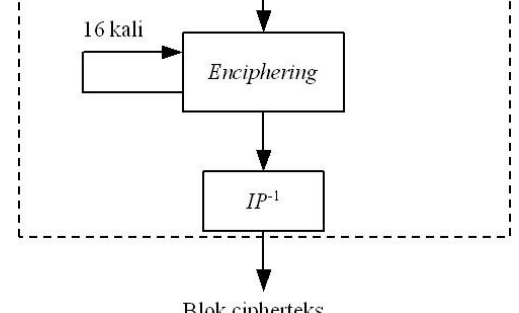
\includegraphics[width=56.70mm,height=86.13mm]{../../images/llm/page_017_img_01.png}%
\end{textblock*}

\end{document}
